\chapter{Model}
Angle and Linear
Explain the two frames and include drawing showing them
Flow of the chapter

\Figref{diagramQuad} shows a representation of the quadcopter where two reference systems, inertial and body, can be seen, as well as the conventions for angles of rotation and forces. \Figref{diagramTorque} shows the body from above and includes the chosen convention for the torques produced by the propellers.

\begin{minipage}{\linewidth}
	\begin{minipage}{0.45\linewidth}
		\begin{figure}[H]
			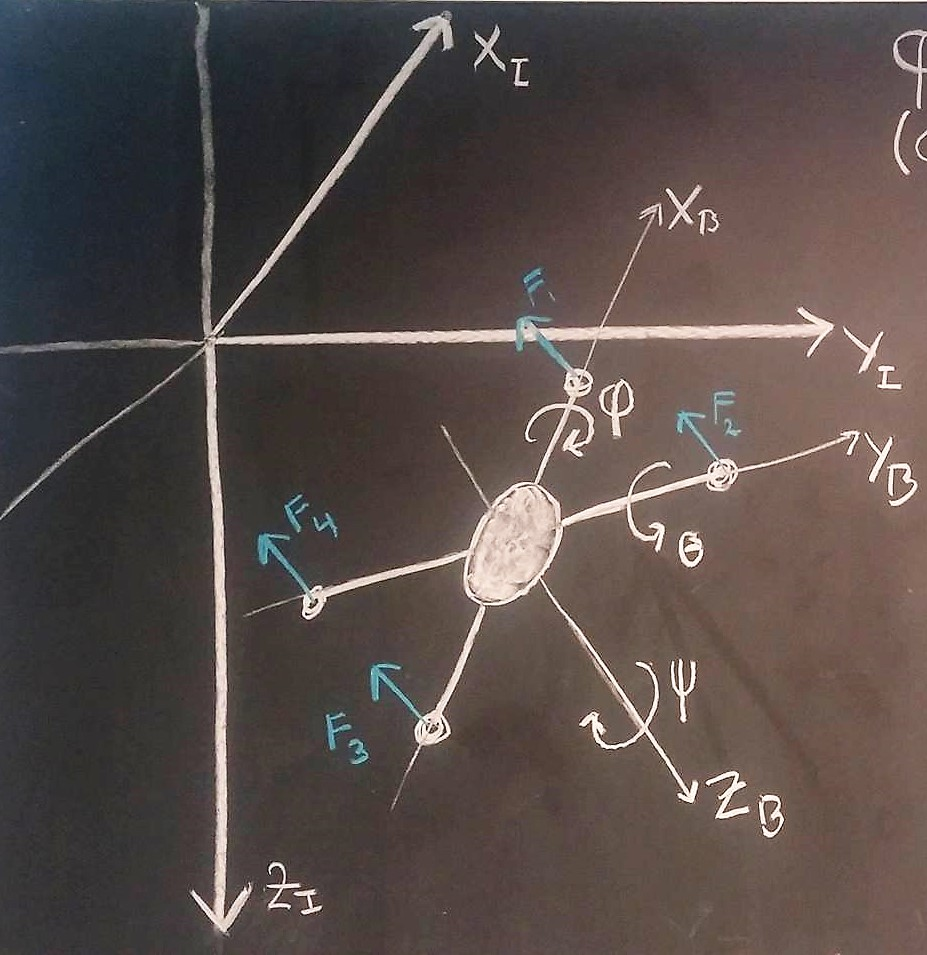
\includegraphics[scale=.27]{figures/drone_diagram}
			\centering
			\captionsetup{justification=centering}
			\captionof{figure}{Diagram of the quadcopter which includes inertial and body reference systems, as well as the references for the angles (roll, pitch and yaw) and the thrust forces produced by the propeller. }
			\label{diagramQuad}
		\end{figure}
	\end{minipage}
	\hspace{0.03\linewidth}
	\begin{minipage}{0.45\linewidth}
		\begin{figure}[H] \vspace{16mm}
			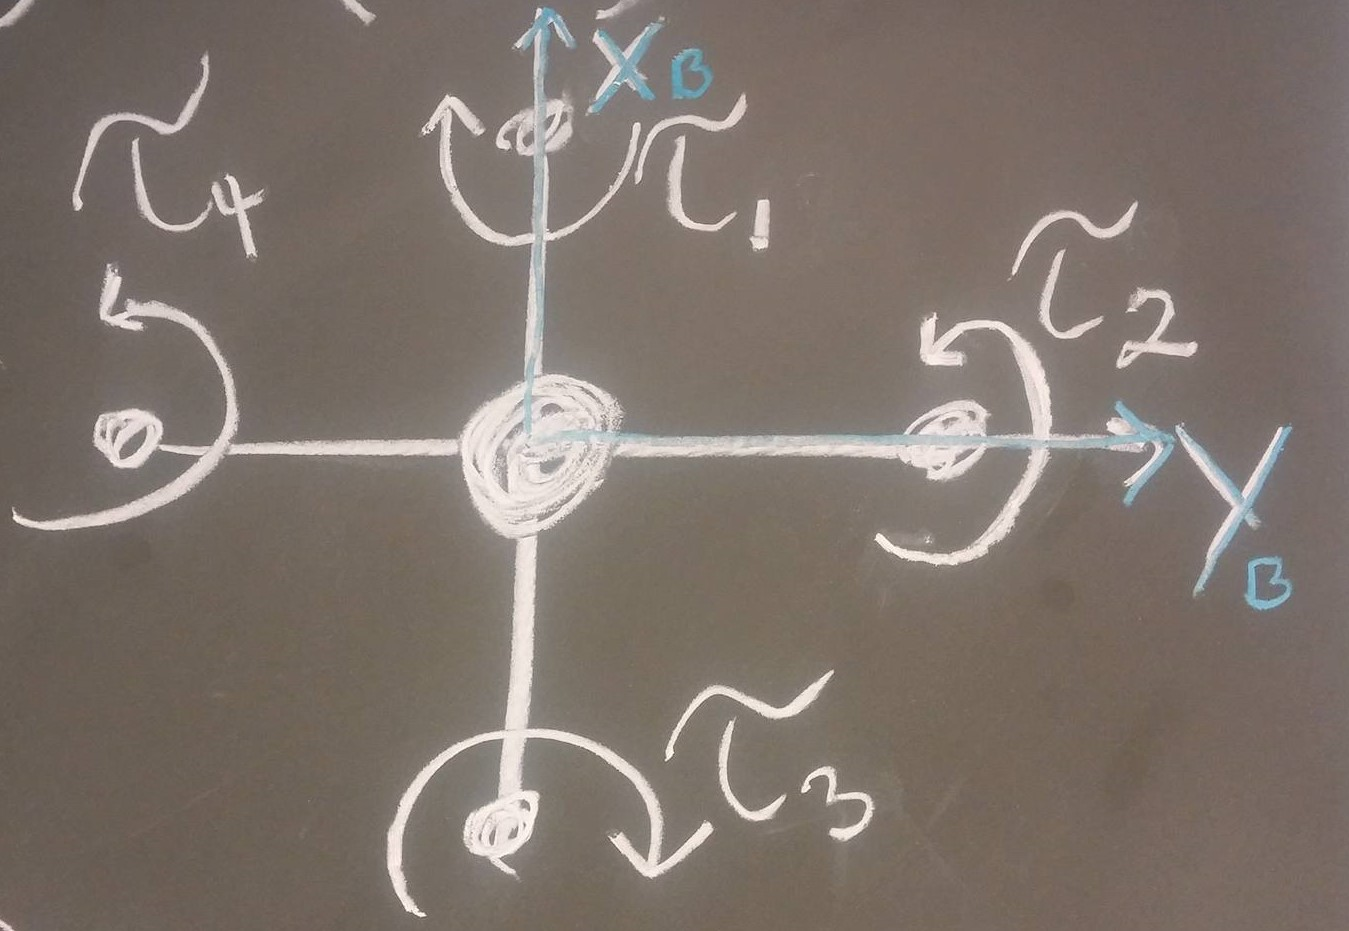
\includegraphics[scale=.18]{figures/torques_diagram}
			\centering
			\captionsetup{justification=centering}
			\captionof{figure}{Diagram of the quadcopter from above, with the references for the torques produced by the drag force at the propeller.}
			\label{diagramTorque}
		\end{figure}
	\end{minipage}
\end{minipage}